\documentclass[12pt]{article}
\usepackage[a4paper,margin=1in]{geometry}
\usepackage{mathptmx}
\usepackage{enumitem}
\usepackage{graphicx}
\setlength{\parindent}{0pt}
\setlength{\parskip}{6pt}
\newcommand{\shead}[1]{\vspace{4pt}\textbf{\underline{#1}}\par}
\pagestyle{plain}

\begin{document}

\begin{center}
\textbf{\itshape A Smart System And Method For The Explainable Detection Of Known
And Zero-Day Network Intrusions Using Hybrid Machine Learning And Anomaly Detection}
\end{center}

\vspace{8pt}

\textbf{Inventor 1:} Kanishk Sigar, Student (B.Tech Student), Department of Computer
Science and Engineering, Graphic Era Hill University, Dehradun, India

\textbf{Inventor 2:} Dr. Mohammad Wazid, Professor, Department of Computer Science and
Engineering, Graphic Era Deemed to be University, Dehradun, India

\textbf{Inventor 3:} Dr. D. P. Singh, Professor and Head, Department of Computer Science
and Engineering, Graphic Era Deemed to be University, Dehradun, India

\vspace{10pt}
\begin{center}\textbf{\underline{INVENTION DISCLOSURE FORMAT}}\end{center}

\shead{a) Invention is Related to:}
This invention is related to the development of a smart system for the explainable
detection of known and previously unseen (zero-day) network intrusions in computer
networks.

Network intrusions refer to any unauthorized or malicious activity that attempts to
compromise the confidentiality, integrity, or availability of a computer network or
its data. These activities can range from denial-of-service and distributed
denial-of-service attacks, port scanning, brute-force attempts, and exploits, to less
obvious forms such as worms, backdoors, reconnaissance, and stealthy data
exfiltration. Regardless of the type of intrusion, a successful attack can have serious
consequences, including financial loss, data theft, service disruption, and damage to
reputation. Unfortunately, this is a global problem that affects individuals,
enterprises, and governments across the world, and it grows more frequent and more
sophisticated as organizations increasingly depend on interconnected systems and the
Internet of Things (IoT).

To address this issue, organizations deploy Intrusion Detection Systems (IDS).
Traditional signature-based systems detect only those attacks for which a known rule
or signature already exists, and therefore cannot detect new or zero-day attacks.
Machine-learning-based systems can detect a wider range of attacks, but they typically
operate as opaque ``black boxes'' that raise an alert without any explanation, which
makes it difficult for a security analyst to trust, verify, and act upon the alert in
time. There is therefore a strong need for an intelligent system that can detect both
known and unknown attacks and, at the same time, clearly explain the reason behind
every detection so that timely and appropriate action can be taken.

To prevent and mitigate this issue, information technology, and in particular machine
learning together with anomaly detection, can play a very vital role in detecting such
intrusions as early as possible and enabling immediate protective action.

\shead{Materials Required:}
Network traffic capturing interface (network tap or port mirroring), a computing system
or server (optionally with a GPU), standard network intrusion datasets for training
(for example, UNSW-NB15 and CIC-IDS2017), and machine learning software libraries.

\shead{b) Novelty of the Invention:}
Following are the novelty components of the proposed system:
\begin{itemize}[leftmargin=1.4em,itemsep=2pt]
  \item The proposed system is a hybrid model that combines three complementary
  detection layers -- a fast signature-rule layer, supervised machine-learning
  classifiers, and a benign-only anomaly detector -- within a single framework.
  \item The benign-only anomaly detector (an autoencoder) is trained only on normal
  traffic and can therefore flag previously unseen (zero-day) attacks without requiring
  any labelled attack data.
  \item Every alert produced by the system is accompanied by an explanation that
  identifies the specific network features responsible for the detection, making the
  system transparent and trustworthy for the security analyst.
  \item It provides explainable detection of both known and unknown attacks within a
  single, deployable application, and can help make networks more secure and reliable.
\end{itemize}

\shead{c) Inventive step of the Invention:}
The novel combination of a signature-rule layer, supervised machine-learning
classifiers, and a benign-only autoencoder-based anomaly detector, together with a
per-alert explanation of every detection using feature-attribution techniques, for the
explainable detection of both known and zero-day network intrusions, is one of the key
inventive steps of this proposed system.

\shead{d) Technical problem solved:}
The proposed system helps in establishing a transparent, trustworthy, and effective
network security mechanism that detects both known and previously unseen attacks while
explaining the reason behind each alert, thereby overcoming the blindness of
signature-only systems and the opacity of conventional machine-learning detectors.

\shead{e) Details of the invention:}
The working of the proposed model is as follows:
\begin{enumerate}[leftmargin=1.6em,itemsep=2pt]
  \item Network traffic flows are captured from the monitored network, and relevant
  statistical features are extracted from each flow.
  \item A feature-preparation pipeline standardizes the numeric features and encodes
  the categorical features into a form suitable for the models.
  \item A signature layer applies fast, human-readable rules to instantly flag obvious
  known-bad flows, such as port scans, brute-force attempts, and data exfiltration.
  \item Supervised machine-learning classifiers (for example, Random Forest and
  XGBoost) analyse the remaining flows and detect known categories of attacks.
  \item A benign-only autoencoder, trained only on normal traffic, computes a
  reconstruction error for each flow; a high reconstruction error indicates an
  anomalous or previously unseen (zero-day) attack.
  \item A decision (fusion) step combines the outputs of the three layers to produce a
  final verdict for each flow.
  \item For every flow flagged as malicious, an explanation module identifies and ranks
  the network features that were most responsible for the decision.
  \item The alert, together with its explanation, is presented to the security analyst
  through an interactive dashboard, so that timely and informed action can be taken.
\end{enumerate}

\shead{f) Applications:}
The proposed system can be embedded very easily into enterprise networks,
Internet-of-Things (IoT) environments, cloud infrastructure, and Security Operations
Centres (SOCs). It gives organizations a safer and more reliable network environment,
and it helps analysts detect, understand, and respond to attacks quickly. Moreover, it
makes network security monitoring more transparent and trustworthy.

\shead{g) Diagram (if any):}
Pictorial representation of the proposed system:

\begin{figure}[h]
\centering
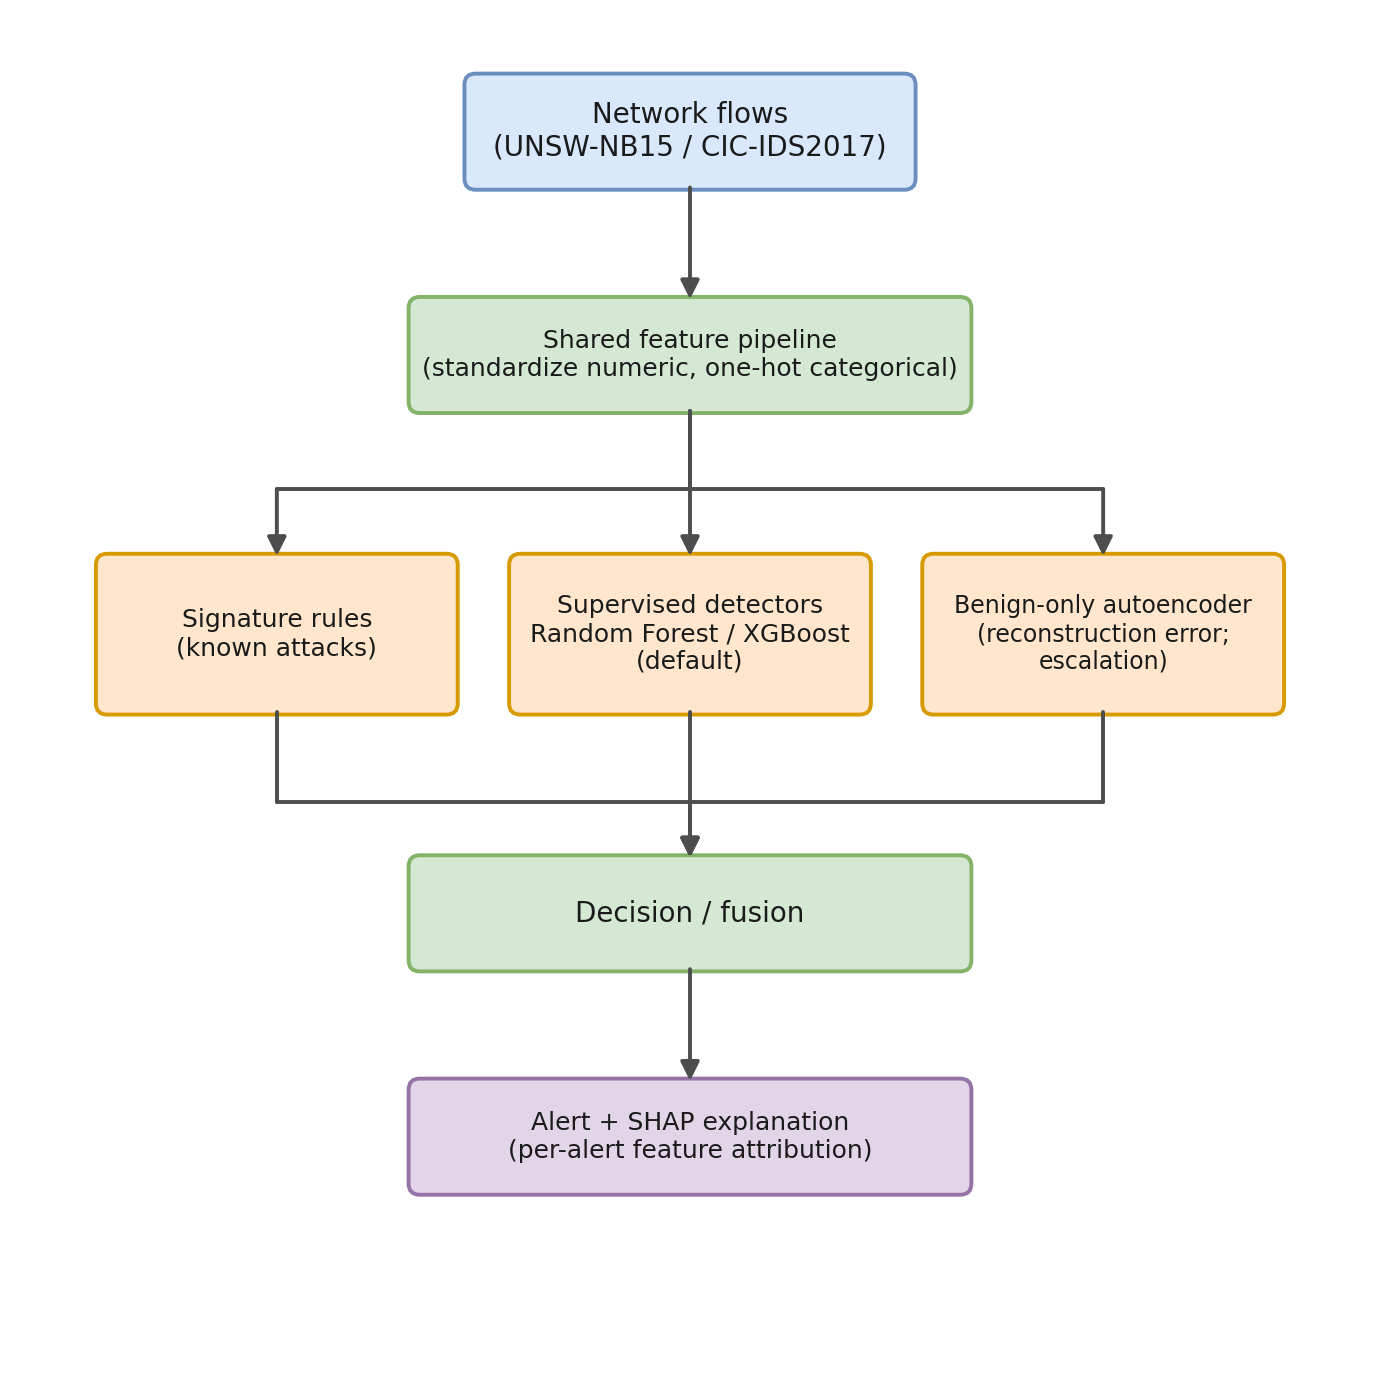
\includegraphics[width=0.95\linewidth]{architecture.png}\\[4pt]
\textbf{Figure 1}: Architecture of the proposed system
\end{figure}

\end{document}
